\documentclass[letterpaper, 11pt]{article}


\usepackage{hyperref}

\usepackage[utf8]{inputenc}
\usepackage{amsmath,amssymb}
\usepackage{graphicx}
\usepackage{caption}
\usepackage{subcaption}
\usepackage{geometry}


%Nueva convenvion para las subfigures es el subcaption package

\usepackage[spanish]{babel}
\usepackage{bm}

\bibliographystyle{alpha}

\leftmargin
\rightmargin

\author{Wilhelm Pablo Karel Zapfe Zaldivar}

%\address{Facultad de Ciencias \\ Ciudad Universitaria \\ México DF}


\begin{document}

\begin{flushright}
Ciudad Universitaria, México, a 23 de octubre del 2013
\end{flushright}
 
\vspace{4cm}
\noindent Facultad de Ciencias
\\ Departameno de Física \\ 
PRESENTE:

\vspace{2cm}

Por este medio presento mi \textbf{INFORME DE ACTIVIDADES} como becario 
número 13256 llevadas a cabo en el proyecto de investigación
CB-101246 a cargo del Dr. David P. Sanders. Mi participación en el proyecto
ha sido desde febrero hasta agosto del 2013, 
comprendiendo una beca
de 7 meses de nivel pos-doctorado, valuada en un total de \$ 101'997 M.N.

Mi trabajo consistió en investigar de forma primordialmente
numérica dos problemas
que compartían configuraciones geométricas similares.
El enfoque primordial de los problemas es encontrar distribuciones y
promedios de los \emph{tiempos de primeros eventos},  
compararlos con derivaciones
teóricas y verificar su posible validez. Una gran parte de mi trabajo
consistió en producir representaciones gráficas adecuadas para
entender situaciones en dimensiones mayores a dos, como
reducciones de espacios de cuatro y tres dimensiones, ya
sea proyecciones o secciones. En este reporte 
usaré dichas ilustraciones para ejemplificar el
trabajo. Además de imágenes estáticas programé 
animaciones para visualizar dinámicamente los problemas, y como
medio de divulgación de ellos. Ellas serán, si lo amerita, usadas
en presentaciones orales 
para público especializado, como congresos y talleres.

La geometría de los problemas es aparentemente simple.
Los elementos dinámicos de los problemas son dos discos
planos, del mismo radio, como se muestra en la primera figura. 
El espacio en el que se pueden mover es un rectángulo plano, es 
decir, el espacio de configuraciones es compacto. La exacta
delimitación del rectángulo es diferente en cada uno de los
problemas, pero no afecta las cualidades geométricas generales.
Los cálculos numéricos en todos los casos fueron hechos con
fronteras de longitud unitaria, es decir, este espacio fue 
concretamente un cuadrado de lado $1$. 

\begin{figure}[h]
  \centering
 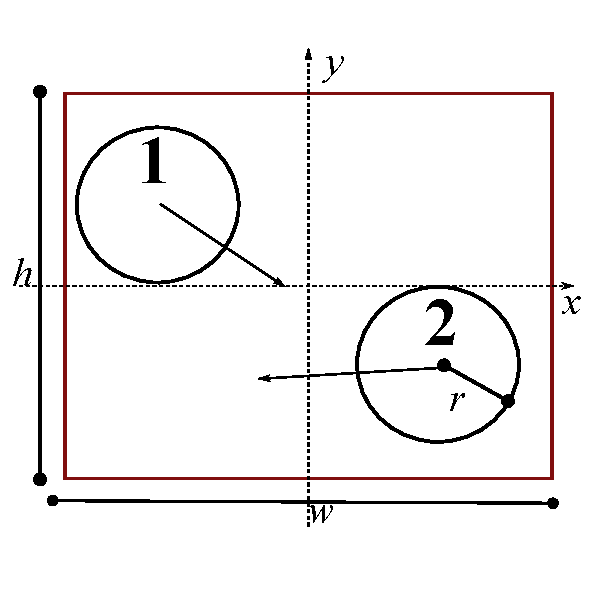
\includegraphics[width=0.55\textwidth]{DiscosenCajaCuadrada01.pdf}
 \caption{La geometría general de los problemas investigados, para propósitos
numéricos, $h=w=1$.}
 \label{PrimeraFigura}
\end{figure}

\section{Caminantes Aleatorios confinados: tiempos de primer encuentro.}

El primer problema planteado fue una extensión mayúscula
 de una investigación
de tiempos de primer encuentro llevada a cabo por 
Sanders \emph{et all} en \cite{SandersLuca}, donde buscaron medidas
promedio de tiempos de encuentro para dos
caminantes aleatorios confinados en una latiz unidimensional.
En dicho trabajo encontraron que el problema
era tratable con métodos de mecánica estadística después de ciertas
simplificaciones de la geometría. 
Mi aportación al problema
era extenderlo para territorios bidimensionales. 
Además de ser la continuación más evidente, el problema
planteado con dos grados de libertad por elemento tiene
mucha mayor riqueza de interpretación.
La motivación original del problema era una tratar de llevar a cabo
un modelo más realista de encuentros de animales territoriales, con posible
aplicación a propagación de epidemias en medios confinados. 
Quisiéramos poder llevar a cabo esta investigación a partir
de primeros principios, sin embargo, puede ser que extender
este modelo a una red de territorios traslapados 
resulte extremadamente difícil de tratar desde el punto
analítico. Planeamos hacer esa tipo de extensión con
más ayuda posteriormente.

El modelo como se mostró en la figura \ref{PrimeraFigura}
es lo suficientemente simple y general como para encontrar muchas 
otras posibles lecturas, como tiempo de libre antes
de una reacción por pares de 
particulas brownianas en un medio líquido. Para un sistema
suficientemente diluido, y condiciones de confinamiento
adecuado, puede dar una respuesta razonable.


Los caminantes aleatorios que ocupan una celda de la latiz son inconvenientes
para generalizaciones de alta dimensión, ya que en el límite 
\emph{continuo} (cuando la finura de la malla de la latiz tiende a cero),
la probabilidad de encuentro se vuelve nula. Esto es debido al número de
dimensiones efectivas del problema, siendo este de cuatro, mientras
que el punto que representa los animales tiende rápidamente
a tener dimensión despreciable, es decir, 
cero (véase la figura \ref{Celdas01}). 
Los caminantes fueron cambiados por discos con un
radio de interacción. Este radio puede representar la distancia mínima
según los cuales los animales pueden interactuar o la infección se 
podría propagar, o, en otras interpretaciones, la distancia mínima para
que una reacción química ocurriera. El centro de los discos
mantendría una dinámica de caminante aleatorio. Esto convierte el problema
en uno de cuatro dimensiones con una geometría sin simetrías, por lo tanto
no reducible. El espacio de configuraciones
 total tiene cuatro dimensiones, que en este caso equivale al espacio
fase del problema, ya que no tenemos velocidades definidas.

\begin{figure}[h]
        \centering
        \begin{subfigure}[b]{0.45\textwidth}
                \centering
                \includegraphics[width=\textwidth]
                                {../epidemias/notas/Celdas_7_con_encuentro.pdf}
                \caption{Celdas Gruesas}
                \label{CGruex}
        \end{subfigure}%
        ~ %add desired spacing between images, e. g. ~, \quad, \qquad etc.
          %(or a blank line to force the subfigure onto a new line)
        \begin{subfigure}[b]{0.45\textwidth}
                \centering
                \includegraphics[width=\textwidth]
                                {../epidemias/notas/Celdas_20_con_encuentro.pdf}
                \caption{Celdas Finas}
                \label{CFinas}
        \end{subfigure}
        ~ %add desired spacing between images, e. g. ~, \quad, \qquad etc.
          %(or a blank line to force the subfigure onto a new line)
        \caption{ Si los caminantes aleatorios se mueven en celdas y
          ocupan solamente una, su límite de encuentro es una linea en
          un espacio cuadridimensional, con probabilidad de encuentro cero 
          (sección tridimensional del espacio
          fase total del problema). }\label{Celdas01}
\end{figure}

Una simple transformación de coordenadas lineal nos
aclara la geometría de ese espacio.
El problema resulta ser dinámicamente equivalente a una partícula
puntual moviendose en un hipercubo con un hipercilíndro atravesado
en diagonal entre dos hiperaristas. Esto es fácil de entender
planteando las condiciones de frontera del problema. Si
denotamos por un índice 1 o 2 respectivamente
las coordenadas verticales y horizontales del centro
de cada disco en la caja, las condiciones que definen el espacio
libre para moverse son que los centros no pueden escapar
del área limitada por el rectángulo y el movimiento
termina cuando los dos discos se encuentran:

\begin{align}
x_1,x_2 \in  & [ -a/2, a/2], \\
y_1\in & [ -b/2, b/2], \\
y_2 = & 0, \\
(x_1-x_2)^2+(y_1-y_2)^2 & \ge (2 r_0)^2.
\end{align}

Una rotación plana 
nos hace ver que la condición de encuentro es cuando 
el punto representante de los centros en el espacio fase
se encuentra contra un cilindro de cuatro dimensiones,
cuyo radio es $\sqrt{2} r_0$.
 La frontera del hipercubo 
es reflejante, mientras que la del cilindro es absorbente. Un diagrama
simplificado de una sección del problema o de un problema
reducido (por ejemplo, fijando la coordenada de la altura de uno de
los dos discos), ayuda a entender un poco la configuración del problema,
véase la figura \ref{CilindroCubo01}. Llevar a cabo la extensión al
caso completo requiere apoyarse en la expresión analítica
de la geometría.

\begin{figure}[h]
  \centering
  \includegraphics[width=0.45\textwidth]
                  {../epidemias/notas/CilindroDiagonal01.png}
                  \caption{Una sección tridimensional del espacio
                    fase completo, mostrando el cilindro absorbente. 
                    La sección se obtiene
                    fijando el valor $y_2=0$.}\label{CilindroCubo01}
\end{figure}

 
En el límite continuo los discos se  comportarían como elemento
de un sistema difusivo, y uno podría pretender resolver el estado
de equilibrio de la ecuación de transporte así obtenida.
Desgraciadamente la forma en que está atravesado el cilindro evita
una descomposición de variables. Después de plantear y analizar
esta situación, mi trabajo consistió en producir los códigos que
llevaran a cabo una investigación numérica de los primeros tiempos
de encuentro y la estadística de esos mismos tiempos,
 de los cuales muestro un ejemplo en la figura \ref{Epidemiastiempo01}. 
Este fue un esfuerzo de programación en paralelo, ya que los muestreos
que se usaron fueron especialmente grandes y nuestro propósito era
obtener una ley general que explicara de forma adecuada el comportamiento
en el rango medio de las geometrías posibles. Para ello usamos
rutinas de paralelización directo en c++ obtenidas por las librerías libres
de openmp y rutinas de muestreos aleatorios de alta calidad provenientes
de la GNU Scientific Library (gsl). Programé rutinas que exploraban
distintas configuraciones de condiciones iniciales no traslapados,
en muestreos grandes, de forma paralela para distintos radios de los
discos. Para radios cercanos al límite la condición no traslapado hacía
lenta la exploración de las condiciones iniciales, así que tuve 
que recurrir a llenados especiales del espacio, que excluyeran zonas
inútiles.




\begin{figure}[h]
  \centering
  \begin{subfigure}[b]{0.45\textwidth}
                \centering
                \includegraphics[width=\textwidth]
                                {../epidemias/animaciones/1030_FirstTimeContagio-PAcumulada.pdf}
                \caption{$r_0=0.42426$}
                \label{Pacum}
        \end{subfigure}%
        ~ %add desired spacing between images, e. g. ~, \quad, \qquad etc.
          %(or a blank line to force the subfigure onto a new line)
        \begin{subfigure}[b]{0.52\textwidth}
                \centering
                \includegraphics[width=\textwidth]
                                {../epidemias/animaciones/MediasIntento01.png}
                \caption{Promedios}
                \label{PProm}
        \end{subfigure}
        ~ %add desired spacing between images, e. g. ~, \quad, \qquad etc.
          %(or a blank line to force the subfigure onto a new line)
        \caption{ Estadística acumulativa de los tiempos
          de primer encuentro. En la primera ilustración vemos un ejemplo de la probabilidad
          acumulada de encuentro para una geometría específica. 
          En el segundo ilustro todos los tiempos promedio de primer
          encuentro como función del radio del disco.}
        \label{Epidemiastiempo01}. 
\end{figure}

Se requeriría un modelo analítico para establecer
una comparación, así que decidimos hacer una simplificación de la geometría
y tratar de resolver el problema difusivo ahí. Tenemos argumentos 
pragmáticos para esperar  que
la solución coincida con los resultados numéricos. Además de ello contamos con
una expresión obtenida por Tejedor \emph{et all} en \cite{TejedorBenichou},
que relaciona tiempos de encuentro en sistemas de caminantes aleatorios con
las características geométricas más simples del problema.
La fórmula obtenida por ellos funciona en el caso no continuo, en 
caminantes unidimensionales. Para poder aplicar esta fórmula y compararla con
la numérica, hicimos una aproximación muy gruesa al problema. Imitando
el razonamiento anterior \cite{SandersLuca} aproximamos el territorio
por un cilindro coaxial con el cilindro de encuentro. 
Dado que tenemos cuatro dimensiones, podemos ajustar el radio y una de las dos
longitudes del hipercilindro que representará al cubo manteniendo área 
absorbente y volumen libre (figura \ref{cilindroeq}). Estos cilindros
son, en el caso general, dos veces coaxiales. 
 También fue mi trabajo encontrar
expresiones exactas para el volumen y el área de estos objetos cuadridimensionales.
La parte realmente tediosa resulta tomar en cuenta la cuña, es decir, 
la parte del cilindro cerca de las aristas del cubo o hipercubo,
cuyo corte transversal a los ejes ya no es circular. 
Las expresiones resultan ser expresiones polinomiales de a lo más
cuarto grado en tres variables: el radio de interacción y 
lo ancho y lo largo del cuadrado del territorio de confinamiento.
Las expresiones resultan ligeramente desagradables, aunque es
fácilmente reconocible las partes de la contribución de la parte
\emph{circular} y la cuña del cilindro.

Dichas cantidades deben usarse para 
producir una geometría equivalente
preservando volumen y área de encuentro 
(el área exterior del cilindro
absorbente, excluyendo la superficie plana de las cuñas). 
Con esta geometría equivalente construimos la versión simplificada
del problema y pretendemos encontrar aquí una solución
difusiva exacta. 
El Dr. Luca Giuggoli buscará la forma de adaptar los resultados
anteriores a esta situación de mayor dimensión. 
Contamos con buenos argumentos para suponer que en realidad,
la extensión será rápidamente obtenible, aunque esto
queda en manos del experto.

\begin{figure}[h]
  \centering
  \includegraphics[width=0.65\textwidth]
                  {../epidemias/notas/CilindroenCilindro01.png}
                  \caption{Una sección tridimensional del concepto de
                    un cilindro equivalente. El cilindro de malla gris
                    tiene el mismo volumen que el cubo. El cilindro
                    de malla azul también tiene el mismo volumen
                    que la frontera absorbente del sistema encierra,
                    más no tiene cuñas en los extremos.
                  }\label{cilindroeq}
                  
\end{figure}



\section{Dos discos rebotando en una caja}

La geometría del problema anterior permite plantear otro problema
cambiando las reglas dinámicas. Sustituyendo la dinámica de caminantes
aleatorios por vuelos libres hamiltonianos, podemos plantear el problema
de un billar de dos discos rebotando dentro de una caja  bidimensional.
Sabemos que dicho sistema es caótico en el sentido fuerte \cite{Sinai70},
sin embargo, 
antes de que efectos promedios como ergodicidad afecten considerablemente
la dinámica, podríamos investigar tiempos de primeros choques y encuentros.
No hay realmente ningún fundamento para pensar que estos tiempos
deben de coincidir con los tiempos promedio que se pueden calcular a partir
de resultados fuertes de teoría ergódica. 
Así que este campo de investigación está aún abierto.

Hay que notar que el espacio fase de este problema tiene dimensión mucho mayor
que el anterior, dado que las coordenadas conjugadas a las posiciones
de los discos son también cambiantes y definidas, 
y la única cantidad conservada del
problema es la energía total, dejándonos todavía con un total de 6 dimensiones
a explorar. La parte de la geometría que es igual al problema anterior
es simplemente el subespacio de configuraciones (espacio de \emph{posiciones}).
Esto implica que hay un volumen de posibilidades a explorar mucho mayor.

Los modelos computacionales que simulan este problema son extensiones del anterior,
así que vale la pena tratar de resolver este problema sin
demasiado esfuerzo. Una ventaja de los
sistemas Hamiltonianos es que, en el caso de pocos grados de libertad,
y donde la mayor parte de la dinámica es vuelo libre, permiten hacer 
simulaciones mucho más rápidas que los sistemas difusivos. La mayor complicación
de este problema es plantear de forma rápida las \emph{condiciones iniciales},
ya que el volumen disponible se pierde más rápidamente que en el caso anterior,
donde permitimos a los centros de los discos llegar hasta las orillas del
territorio, lo cual no es aceptable en este caso. 
Una vez resuelta esta 
dificultad, uno puede obtener distribuciones acumuladas de tiempos
de primer encuentro, como se muestran en la figura \ref{BillarTiempo01}.


\begin{figure}[h]
  \centering
  \begin{subfigure}[b]{0.49\textwidth}
                \centering
                \includegraphics[width=\textwidth]
                                {../TwoDiskinaRectangle/FirstChoqueEstadistica/1015_FirstTimeChoque-PAcumulada.pdf}
                \caption{$r_0=0.09186$}
                \label{PacumHam}
        \end{subfigure}%
        ~ %add desired spacing between images, e. g. ~, \quad, \qquad etc.
          %(or a blank line to force the subfigure onto a new line)
        \begin{subfigure}[b]{0.49\textwidth}
                \centering
                \includegraphics[width=\textwidth]
                {../TwoDiskinaRectangle/FirstChoqueEstadistica/TiemposMedios01.pdf}
                \caption{Promedios}
                \label{PPromHam}
        \end{subfigure}
        ~ %add desired spacing between images, e. g. ~, \quad, \qquad etc.
          %(or a blank line to force the subfigure onto a new line)
        \caption{La misma estadística de tiempos de primer encuentro mostrada en la figura 
        \ref{Epidemiastiempo01}, pero con dinámica hamiltoniana. Nótese lo diferente
        de las distribuciones. }
        \label{BillarTiempo01}. 
\end{figure}

Para poder comparar los efectos de las reglas dinámicas en cada uno
de los dos problemas, escogí una \emph{normalización} de la escala
temporal que permita llevar a cabo al menos una comparación cualitativa
de las distribuciones acumuladas de tiempos de primer encuentro. 
El pequeño truco es el siguiente: dado que en el caso hamiltoniano
la energía total sólo afecta como factor de escala, puedo escoger
el valor de ésta como aquel que produce velocidades promedio
de cada uno de los dos discos de magnitud unitaria, es decir,
que recorran una unidad de distancia en una unidad de tiempo. 
Para simplificar esto, también fijo la masa de los discos en 
una unidad numérica abstracta. En el caso difusivo esto equivale
a multiplicar el tiempo discreto de pasos en celdas de los
caminantes aleatorios por la longitud de la celda, de forma
que la velocidad instantánea del centro del disco sea
también unitaria (recorrería una unidad de distancia en un
tiempo de una unidad también, cada uno). Esto fija un criterio
para la comparación, más no es suficiente. El radio total de
los discos no es buena medida de comparación, dado que en el caso
hamiltoniano y en el caso aleatorio hemos escogido
criterios distintos de confinameniento. Esto se puede corregir
simplemente cambiando el segundo caso a moverse con los radios
de interacción \emph{dentro de la frontera}, lo cual,
sin embargo, resulta incómodo para las interpretaciones que hemos
buscado. Así que creo que el criterio más adecuado para la comparación
es la del \emph{Volumen libre}, es decir, el espacio
que tiene la partícula en el espacio de configuración total 
para moverse. Es por eso que muestro figuras de radios distintos
en los dos casos.
Aún hay algo más: el cambio de distribución
puede deberse no a las reglas dinámicas, sino a las cuatro
dimensiones extra que tiene el espacio fase del sistema
hamiltoniano: los momentos lineales de cada disco.  

Esta investigación promete ser de interés para la 
comunidad que estudia billares caóticos,
como demuestran artículos publicado recientemente \cite{Munakata02}.
Es, hasta donde nuestro conocimiento alcanza, original. Las fórmulas teóricos
que nos permitirán establecer la validez de nuestros resultados serán
adaptaciones originales de resultados obtenidos por teoría ergódica. 
Esperamos contar pronto 
con una primera versión de un artículo publicable al respecto.

\vfill

\begin{tabular}{cc}
Becario &  Vo. Bo. Responsable del Proyecto.\\
\includegraphics[width=0.2\textwidth]{../../papeleogeneral/Firma01.png} &  \\
Dr. Wilhelm P. K. Zapfe Zaldivar  & Dr. David. P. Sanders
\end{tabular}


\newpage
\bibliography{General.bib}


\end{document}
